% !TeX program = xelatex
\documentclass[aspectratio=169]{beamer}
% Overleaf 共用导言区：Fandol 字体，不依赖仓库内字体文件
% 纯文字版：不加载 TikZ 绘图库和代码高亮配置

\usepackage{fontspec}
\usepackage{xeCJK}

% Overleaf 自带 Fandol 字体，避免上传 44 MB 的 LXGW / Sarasa 字体
\setCJKsansfont{FandolHei}[BoldFont=FandolHei-Bold]
\setCJKmainfont{FandolSong}[
  BoldFont=FandolSong-Bold,
  ItalicFont=FandolKai,
  BoldItalicFont=FandolKai
]
\setCJKmonofont{FandolFang}

% Overleaf 的 TeX Live 自带 TeX Gyre，替代 Windows 的 Times New Roman / Arial
\setmainfont{TeX Gyre Termes}
\setsansfont{TeX Gyre Heros}

\usetheme{SDU}

\usepackage{amsmath,amssymb}
\usepackage{booktabs}
\usepackage{multicol}

\hypersetup{colorlinks=true,linkcolor=.,citecolor=peaking,urlcolor=peaking!70!black}

% 关闭导航符号，保留主题的顶部进度条与页脚
\setbeamertemplate{navigation symbols}{}

% 常用小工具
\newcommand{\hl}[1]{\textcolor{peaking}{\textbf{#1}}}
\newcommand{\luogu}[2]{\href{https://www.luogu.com.cn/problem/#1}{\texttt{#1}\,\textnormal{#2}}}


% 不自动插入目录页
\AtBeginSection[]{}
\AtBeginSubsection[]{}

\title{常见优化方法（二）}
\date{2026 年 11 月}

\begin{document}

\begin{frame}
    \titlepage
\end{frame}

% ============================================================
\section{离散化}

\begin{frame}{离散化：只保留相对大小}
    \begin{columns}[T]
        \begin{column}{0.50\textwidth}
            \small
            原始值可能很大、很稀疏，例如
            \[
                10,\ 1000,\ 10^9,\ 42,
            \]
            但我们只关心它们谁大谁小。

            \vspace{0.4em}
            \hl{离散化}：把原始值映射成排名 $1\sim k$，并保持\\
            $x<y \iff \operatorname{rank}(x)<\operatorname{rank}(y)$
            \begin{itemize}
                \item 排序、去重
                \item 时间 $O(n\log n)$
                \item 之后就能用数组、桶、其他数据结构等维护
            \end{itemize}
        \end{column}
        \begin{column}{0.46\textwidth}
            \begin{exampleblock}{举例}
                \footnotesize
                原值：$10,1000,10^9,42$。\\
                排序：$10,42,1000,10^9$。\\
                排名：$1,2,3,4$。\\
                原来 $42<1000$，离散化后 $2<3$，大小关系不变。
            \end{exampleblock}
            \vspace{0.4em}
            \footnotesize
            只保留相对大小，不保留原值之间的间隔。
        \end{column}
    \end{columns}
\end{frame}

\begin{frame}{例题 F：P1496 火烧赤壁}
    \begin{columns}[T]
        \begin{column}{0.51\textwidth}
            \small
            \luogu{P1496}{火烧赤壁}
            \begin{block}{题意}
                \footnotesize
                给出 $n$ 个着火区间 $[a,b)$，求燃烧位置的总长度。
                区间可能重叠。
            \end{block}
            \begin{itemize}
                \item $n\le 2\times10^4$
                \item 坐标 $|a|,|b|<2^{31}$，不能开布尔数组
                \item 把所有端点离散化，在排名上做差分
            \end{itemize}
        \end{column}
        \begin{column}{0.45\textwidth}
            \begin{block}{算法}
                \footnotesize
                \begin{enumerate}
                    \item 收集所有 $a,b$，排序去重得到 $x_1<\dots<x_k$
                    \item 每个区间对应排名 $[L,R)$
                    \item 差分：\texttt{d[L]++, d[R]--}
                    \item 扫描相邻排名：若覆盖数 $>0$，累加 $x_{i+1}-x_i$
                \end{enumerate}
            \end{block}
        \end{column}
    \end{columns}
\end{frame}

% ============================================================
\section{单调队列}

\begin{frame}{单调队列：从一个例子说起}
    \textbf{问题：}数组 $a=(1,3,-1,-3,5,3,6,7)$，
    有一个长度为 $k=3$ 的滑动窗口从左到右滑动，
    求每个窗口的最小值。\\
    \vspace{0.3em}
    暴力：每个窗口扫一遍，$O(nk)$。\\
    \vspace{0.3em}
    窗口每次只进入一个数，只离开一个数，能否利用？\\
    \vspace{1em}
    这就是接下来要讲到的单调队列。单调队列实际上是一种双端队列，仍然可以
    队尾插入、队首弹出，但是也可以进行队尾弹出（“插队”）。
\end{frame}

\begin{frame}{单调队列：从一个例子说起}
    \begin{columns}[T]
        \begin{column}{0.50\textwidth}
            \small
            $a=(1,3,-1,-3,5,3,6,7)$，$k=3$\\
            \vspace{0.3em}
            用双端队列存\hl{下标}，逐元素处理：
            \begin{itemize}
                \item $i=0,\ a_0=1$：队空，入队 $\to [\,0\,]$
                \item $i=1,\ a_1=3$：$1<3$，入队 $\to [\,0,1\,]$
                \item $i=2,\ a_2=-1$：\\
                    {
                       队尾 $a_1=3\ge -1$，弹；\\
                       队尾 $a_0=1\ge -1$，弹；\\
                       入队 $\to [\,2\,]$。窗口 $[0,2]$ 最小值 $-1$。
                    }
            \end{itemize}
            \vspace{0.3em}
            \textbf{疑问：}为什么 $-1$ 一进来，
            就能把 $1$ 和 $3$ 都弹掉？为什么能这样维护？
        \end{column}
        \begin{column}{0.46\textwidth}
            \begin{exampleblock}{队列中的值}
                \footnotesize
                \begin{tabular}{c|c|c}
                    $i$ & $a_i$ & 队列（值）\\\hline
                    0 & $1$  & $1$ \\
                    1 & $3$  & $1,\,3$ \\
                    2 & $-1$ & $-1$ \\
                    3 & $-3$ & $-3$ \\
                    4 & $5$  & $-3,\,5$ \\
                    5 & $3$  & $-3,\,3$ \\
                    6 & $6$  & $3,\,6$ \\
                    7 & $7$  & $3,\,6,\,7$ \\
                \end{tabular}
            \end{exampleblock}
            \footnotesize
            队列里的值始终\hl{单调递增}，队首恰是当前窗口最小值。
        \end{column}
    \end{columns}
\end{frame}

\begin{frame}{为什么队尾淘汰是对的？}
    \begin{columns}[T]
        \begin{column}{0.50\textwidth}
            \small
            新来的元素 $x$ 又\textbf{比队尾小}、
            又\textbf{排得更靠右}（所以也走得更晚），
            那队尾就\textbf{彻底没用了}。

            \vspace{0.4em}
            \textbf{为什么？}看队尾那个下标 $p$，再看新来的 $i$。
            \begin{itemize}
                \item 窗口是\textbf{连续}的一段，而且往\textbf{右}滑；
                \item $i$ 在 $p$ 的右边，所以——
                      \textbf{之后}哪个窗口还包含 $p$，
                      那个窗口就\textbf{也一定包含 $i$}；
                \item 而 $a_i\le a_p$，
                      所以那个窗口的最小值\textbf{轮不到} $p$。
            \end{itemize}

            \vspace{0.3em}
            \hl{能用的窗口全被 $i$ 覆盖，值还更小}\\
            $\Rightarrow$ $p$ 永远当不了最小值，\hl{可以放心弹}。

            \vspace{0.3em}
            于是：队尾比 $i$ 大/相等就弹，
            弹到比 $i$ 小为止，然后 $i$ 入队。
        \end{column}
        \begin{column}{0.46\textwidth}
            \begin{exampleblock}{举例：$a=(1,3,-1)$，$k=3$}
                \footnotesize
                现在队列里是 $1,\,3$（下标 $0,1$）。\\
                新来的是 $-1$（下标 $2$）。

                \vspace{0.3em}
                $3>-1$，且 $3$ 在 $-1$ 左边。\\
                以后包含下标 $1$ 的窗口，
                比如 $[0,1,2]$、$[1,2,3]$，一定也含下标 $2$；\\
                里面既有 $3$ 又有 $-1$，最小值不是 $3$。\\
                所以 $3$ 不可能是答案了，弹走。

                \vspace{0.3em}
                同理，之后 $1$ 也被弹走，队列变空，$-1$ 入队。\\
                窗口 $[0,2]$ 的最小值就是 $-1$。
            \end{exampleblock}
        \end{column}
    \end{columns}
\end{frame}

\begin{frame}{单调队列：滑动窗口的最值}
    窗口 $[i-k+1,i]$ 向右滑动，要求每个窗口的最小值。

    \vspace{0.4em}
    用双端队列存\hl{下标}：
    \begin{itemize}
        \item 队首过期：\texttt{q[head] <= i-k} 就弹出
        \item 队尾淘汰：\texttt{a[q[tail]] >= a[i]} 就弹出
        \item 当前元素入队，队首即窗口最小值
    \end{itemize}
    \vspace{0.4em}
    每个下标最多进队、出队一次，总复杂度 $O(n)$。
\end{frame}

\begin{frame}{例题 G：P1886 滑动窗口}
    \begin{columns}[T]
        \begin{column}{0.50\textwidth}
            \small
            \luogu{P1886}{【模板】单调队列}
            \begin{block}{题意}
                \footnotesize
                长度为 $n$ 的序列，窗口大小 $k$ 从左向右滑动。
                输出每个窗口的最小值、最大值各一行。
            \end{block}
            \begin{itemize}
                \item $n\le 10^6$
                \item 暴力每窗扫 $k$ 个：$O(nk)$
                \item 单调队列：$O(n)$
            \end{itemize}
        \end{column}
        \begin{column}{0.46\textwidth}
            \begin{block}{步骤}
                \footnotesize
                \begin{enumerate}
                    \item 先做最小值：队首过期就弹出
                    \item 队尾比当前元素大就弹出
                    \item 当前下标入队，输出队首
                    \item 最大值把比较方向反过来，再做一遍
                \end{enumerate}
            \end{block}
        \end{column}
    \end{columns}
\end{frame}

% ============================================================
\section{倍增：ST 表}

\begin{frame}{倍增：用 $2$ 的幂次加速}
    \begin{columns}[T]
        \begin{column}{0.50\textwidth}
            \small
            任何一个整数都能拆成若干个 $2$ 的幂之和：
            \[
                13=8+4+1.
            \]
            \hl{倍增}就是预处理 $2^j$ 一级的信息，
            查询时用二进制拆分快速组合。

            \vspace{0.5em}
            两种常见形态：
            \begin{enumerate}
                \item \hl{区间倍增}：ST 表，静态区间最值
                \item \hl{树上倍增}：LCA，$2^j$ 级祖先
            \end{enumerate}
        \end{column}
        \begin{column}{0.46\textwidth}
            \begin{exampleblock}{举例}
                \footnotesize
                先预处理长度为 $1,2,4,8$ 的答案；\\
                查询长度 $13$ 时，拆成 $8+4+1$，\\
                把三段预处理结果合并即可。
            \end{exampleblock}
            \vspace{0.4em}
            \footnotesize
            预处理通常 $O(n\log n)$，单次查询 $O(1)$ 或 $O(\log n)$。
        \end{column}
    \end{columns}
\end{frame}

\begin{frame}{ST 表：$O(n\log n)$ 预处理，$O(1)$ 查询}
    \begin{columns}[T]
        \begin{column}{0.50\textwidth}
            \small
            设以 $i$ 为左端点，长度为 $2^j$ 的区间的答案：
            \[
                f_{i,j}=\max\{a_i,\dots,a_{i+2^j-1}\}.
            \]
            边界与转移：
            \[
                f_{i,0}=a_i,\qquad
                f_{i,j}=\max\left(f_{i,j-1},f_{i+2^{j-1},j-1}\right).
            \]
            长度为 $1$ 的区间答案就是这个数本身。\\
            长度为 $2^j$ 的区间答案是两个 $2^{j-1}$ 长度区间的答案取最大。\\
            查询 $[l,r]$，令 $k=\lfloor\log_2(r-l+1)\rfloor$：
            \[
                \max\left(f_{l,k},f_{r-2^k+1,k}\right).
            \]
            找到两个可以覆盖询问的区间，取最大。
        \end{column}
        \begin{column}{0.46\textwidth}
            \begin{exampleblock}{举例}
                \footnotesize
                查询 $[2,7]$，长度 $6$，$k=2$，块长为 $4$。\\
                块 1 为 $[2,5]$，块 2 为 $[4,7]$。\\
                两块覆盖整个区间，重叠的 $[4,5]$ 不影响最大值。
            \end{exampleblock}
            \vspace{0.4em}
            \footnotesize
            只适用于\hl{可重复贡献}的运算：max/min/gcd。\\
            区间和不能用，因为重叠部分会被算两次。\\
            \vspace{1em}
            注：ST = Sparse Table，稀疏表。
        \end{column}
    \end{columns}
\end{frame}

\begin{frame}{例题 H：P3865 ST 表}
    \begin{columns}[T]
        \begin{column}{0.50\textwidth}
            \small
            \luogu{P3865}{【模板】ST 表}
            \begin{block}{题意}
                \footnotesize
                给定长度为 $N$ 的数列，回答 $M$ 次
                “区间最大值”询问。
            \end{block}
            \begin{itemize}
                \item $N\le 10^5$，$M\le 2\times10^6$
                \item 时限只有 $0.8$ 秒
                \item 必须 $O(1)$ 查询
            \end{itemize}
        \end{column}
        \begin{column}{0.46\textwidth}
            \begin{block}{步骤}
                \footnotesize
                \begin{enumerate}
                    \item 预处理 ST 表
                    \item $f_{i,0}=a_i$
                    \item 按 $j=1,2,\dots$ 递推 $f_{i,j}$
                    \item 每次询问用两个长度为 $2^k$ 的块合并
                \end{enumerate}
            \end{block}
            \vspace{0.4em}
            \footnotesize
            $M$ 很大，输入输出都要注意效率。
        \end{column}
    \end{columns}
\end{frame}

% ============================================================
\section{倍增：LCA}

\begin{frame}{LCA：树上倍增}
    \begin{columns}[T]
        \begin{column}{0.51\textwidth}
            \small
            有根树中，$u,v$ 的最近公共祖先记作 $\operatorname{LCA}(u,v)$。

            \vspace{0.3em}
            预处理 $f_{u,j}$：$u$ 的 $2^j$ 级祖先。
            \[
                f_{u,0}=parent(u),\qquad
                f_{u,j}=f_{f_{u,j-1},j-1}.
            \]
            查询步骤：
            \begin{enumerate}
                \item 把较深的点抬到同一深度
                \item 若两点相同，返回该点
                \item 从高位到低位同时抬，若祖先不同就抬
                \item 返回 $f_{u,0}$
            \end{enumerate}
            \footnotesize
            单次 $O(\log n)$，预处理 $O(n\log n)$。\\
            注：LCA = Lowest Common Ancestor。
        \end{column}
        \begin{column}{0.45\textwidth}
            \begin{exampleblock}{举例}
                \centering
                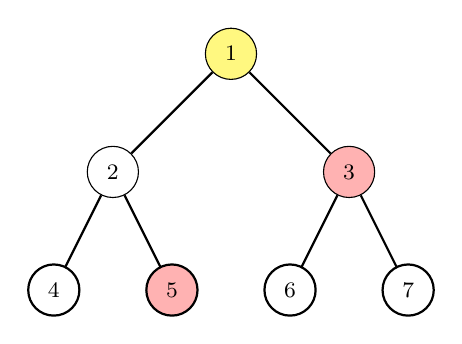
\begin{tikzpicture}[
                    every node/.style={circle,draw,minimum size=6.5mm,
                                       inner sep=0pt,font=\footnotesize},
                    level 1/.style={sibling distance=30mm},
                    level 2/.style={sibling distance=15mm},
                    edge from parent/.style={draw,thick}
                ]
                    \node[fill=yellow!50] {1}
                        child {node {2}
                            child {node {4}}
                            child {node[fill=red!30] {5}}
                        }
                        child {node[fill=red!30] {3}
                           child {node {6}}
                            child {node {7}}
                        };
                \end{tikzpicture}

                \vspace{0.6em}
                \footnotesize
                红点 $5,3$ 的最近公共祖先：\\
                黄点 $1$。
            \end{exampleblock}
        \end{column}
    \end{columns}
\end{frame}

\begin{frame}{例题 I：P3379 LCA}
    \begin{columns}[T]
        \begin{column}{0.48\textwidth}
            \small
            \luogu{P3379}{【模板】最近公共祖先}
            \begin{block}{题意}
                \footnotesize
                给定一棵 $n$ 个点的有根树，根为 $s$，
                回答 $q$ 次询问：$u,v$ 的 LCA。
            \end{block}
            \begin{itemize}
                \item $n,q\le 5\times10^5$
                \item 倍增：$O((n+q)\log n)$
            \end{itemize}
        \end{column}
        \begin{column}{0.48\textwidth}
            \begin{block}{步骤}
                \footnotesize
                \begin{enumerate}
                    \item 建邻接表，从根 DFS，求 $dep$ 和 $f_{u,0}$
                    \item 按 $j=1\dots \lfloor\log_2 n\rfloor$ 递推 $f_{u,j}$
                    \item 每次询问：抬到同深度 $\to$ 同时抬 $\to$ 返回父亲
                \end{enumerate}
            \end{block}
            \vspace{0.4em}
        \end{column}
    \end{columns}
\end{frame}

% ============================================================
\section{小结}

\begin{frame}{本讲小结}
    \centering
    \footnotesize
    \begin{tabular}{llll}
        \toprule
        方法 & 应用 & 复杂度 & 例题 \\
        \midrule
        离散化 & 值域大、只用相对大小 & $O(n\log n)$ & P1496 \\
        单调队列 & 滑动窗口最值 & $O(n)$ & P1886 \\
        ST 表 & 静态区间最值、可重复贡献 & $O(n\log n)/O(1)$ & P3865 \\
        树上倍增 & 最近公共祖先、$2^j$ 级祖先 & $O((n+q)\log n)$ & P3379 \\
        \bottomrule
    \end{tabular}
    \vspace{1.1em}
    \begin{block}{题单}
        \footnotesize
        完成题单 $\#3$ 里的所有题目
    \end{block}
\end{frame}

\end{document}
